\documentclass[conference]{IEEEtran}
\IEEEoverridecommandlockouts
% The preceding line is only needed to identify funding in the first footnote. If that is unneeded, please comment it out.
\usepackage{cite}
\usepackage{amsmath,amssymb,amsfonts}
\usepackage{algorithmic}
\usepackage{graphicx}
\usepackage{textcomp}
\usepackage{xcolor}
\usepackage{listings}
\def\BibTeX{{\rm B\kern-.05em{\sc i\kern-.025em b}\kern-.08em
    T\kern-.1667em\lower.7ex\hbox{E}\kern-.125emX}}
	
	
	
%Customize a bit the look
\lstset{ %
backgroundcolor=\color{white}, % choose the background color; you must add \usepackage{color} or \usepackage{xcolor}
basicstyle=\footnotesize, % the size of the fonts that are used for the code
breakatwhitespace=false, % sets if automatic breaks should only happen at whitespace
breaklines=true, % sets automatic line breaking
captionpos=b, % sets the caption-position to bottom
commentstyle=\color{mygreen}, % comment style
deletekeywords={...}, % if you want to delete keywords from the given language
escapeinside={\%*}{*)}, % if you want to add LaTeX within your code
extendedchars=true, % lets you use non-ASCII characters; for 8-bits encodings only, does not work with UTF-8
frame=single, % adds a frame around the code
keepspaces=true, % keeps spaces in text, useful for keeping indentation of code (possibly needs columns=flexible)
keywordstyle=\color{blue}, % keyword style
% language=Octave, % the language of the code
morekeywords={*,...}, % if you want to add more keywords to the set
numbers=left, % where to put the line-numbers; possible values are (none, left, right)
numbersep=5pt, % how far the line-numbers are from the code
numberstyle=\tiny\color{mygray}, % the style that is used for the line-numbers
rulecolor=\color{black}, % if not set, the frame-color may be changed on line-breaks within not-black text (e.g. comments (green here))
showspaces=false, % show spaces everywhere adding particular underscores; it overrides 'showstringspaces'
showstringspaces=false, % underline spaces within strings only
showtabs=false, % show tabs within strings adding particular underscores
stepnumber=1, % the step between two line-numbers. If it's 1, each line will be numbered
stringstyle=\color{mymauve}, % string literal style
tabsize=2, % sets default tabsize to 2 spaces
title=\lstname % show the filename of files included with \lstinputlisting; also try caption instead of title
}

\definecolor{darkgray}{rgb}{.4,.4,.4}
\definecolor{purple}{rgb}{0.65, 0.12, 0.82}

\lstdefinelanguage{JavaScript}{
keywords={typeof, new, true, false, catch, function, return, null, catch, switch, var, if, in, while, do, else, case, break},
keywordstyle=\color{blue}\bfseries,
ndkeywords={class, export, boolean, throw, implements, import, this},
ndkeywordstyle=\color{darkgray}\bfseries,
identifierstyle=\color{black},
sensitive=false,
comment=[l]{//},
morecomment=[s]{/*}{*/},
commentstyle=\color{purple}\ttfamily,
stringstyle=\color{red}\ttfamily,
morestring=[b]',
morestring=[b]"
}

\lstset{
language=JavaScript,
extendedchars=true,
basicstyle=\footnotesize\ttfamily,
showstringspaces=false,
showspaces=false,
numbers=left,
numberstyle=\footnotesize,
numbersep=9pt,
tabsize=2,
breaklines=true,
showtabs=false,
captionpos=b,
linewidth=.46\textwidth,
xleftmargin=.2cm
}
	
\begin{document}

\title{Testing Methodologies for Asynchronous Centralized Simulations\\
}

\author{\IEEEauthorblockN{Sorin Badila, Cale Campbell, Ryan Wilk}
\IEEEauthorblockA{\textit{Department of Computer Science and Engineering} \\
\textit{Oakland University}\\
Rochester, United States \\
sfbadila@oakland.edu, ccampbell5@oakland.edu, rmwilk@oakland.edu}
}

\maketitle

\begin{abstract}
 Distributed interactive multi-body simulations are an increasingly prevalent breed of software and demand unique strategies with respect to testing. 
 Classically non-networked multiplayer video gaming takes place on a single machine hosting a single local environment within which all players directly 
 control actors in a simulation. Modern networked gaming often requires that a singular environment be remotely hosted with all player-controlled actors and 
 their interactions be distributed to connected client applications. With all these simulations, it is paramount that the individual units in the simulations 
 as well as all the moving parts in the server are rigorously tested. The research gathered for this paper will outline the testing methodologies that we find 
 to be the most significant. Combining strong unit and integration testing inside the server, each simulation needs to be tested for usability, compatibility, and 
 reliability. Likewise, since the integrity of the simulation is paramount, susceptibility to malicious or incorrect information fed into the system  must be mitigated, 
 and as such, we will explore mechanisms by which test the system.

\end{abstract}

\begin{IEEEkeywords}
Testing, Nodejs, networking, multiplayer, WebSocket, software engineering
\end{IEEEkeywords}

\section{Introduction}
In our work we aim to create a testing framework for centralized simulations serving one or more clients concurrently. In order to accomplish the goal of serving
multiple clients concurrently and in a timely manner, the server must communicate with the clients in an asynchronous manner in that there can be no reliance 
on confirming whether a data packet was received successfully, the server simply broadcasts any updates to the simulation state to all clients. With these considerations
in mind, any rigorous and complete testing must account for these features. We will be introducing a number of different approaches with which to build a complete, end to end
testing framework which can be used to ensure the correctness and completeness of any system utilizing a centralized simulation.

Unit testing can be achieved through traditional means of subjecting applicable functions to predetermined inputs and comparing their results to expected results. 
Functional testing presents a less straight-forward solution. For example, instead of treating testing in the traditional sense of invoking one method at a time,
we can designate a certain action within the game to be the target of functional testing. Taking it one step further, we have the end-goal of automating such a process such that 
it can be invoked with little operator input, akin to how a set of unit tests would function. In order to acomplish the task of automation, we will provide solutions to the problem
of asynchronicity.

In the latter half of the paper, we will be introducing an actual instance of such a simulation, a browser-based online multiplayer javascript application called NodeTank. 
This application involves two primary components, a server, and one or more connected clients. Each client instance renders the game environment to the players as well as a tank object which accepts control inputs from 
a player. Client instances are responsible for forwarding control inputs to the server. The server is responsible for tracking and maintaining state information relevant 
to the gameplay. Various examples of state include health status, position, and orientation. This information needs to be forwarded from the server to the client applications 
with minimal latency in order to provide a continuous stream of snapshots of the game’s state. Client applications are also responsible for recreating and displaying this 
information for the player with the end-goal of providing all players with consistent up-to-date information. We will apply the framework concepts developed in the former sections to this 
case study to demonstrate its efficacy.

\section{Related Works}

The works of Ariurek et al[2] are very interesting to our research because they propose several mechanisms by which to introduce automated test agents into the game
development cycle with the goal of finding defects. They have proposed two mechanisms by which to facilitate this automation; human-like agents and synthetic agents. 
A human-like agent is a separate program which learns the rules and behavior of a game via reinforcement learning. With reinforcement learning, this type of agent would 
learn how a human would play the game as it would have the same reward incentive as a human player, and is thus likely to detect defects which are similar in nature to those 
detected by humans. Their proposed synthetic agent is also a type of program which is trained via reinforcement learning, except its goals are not inline with the goals of a 
real human player. For example, a synthetic agent could be rewarded with implementing a scenario which would be detrimental to winning the game, but which would be likely to
reveal a defect otherwise hidden from expected behavior. Using both of these methods, Ariurek et al have created a system in which the quality of a game could be tested automatically 
and not in a predetermined fashion. 

Rezin et al[3] developed a model checking mechanism for a specific multiplayer game. They did so by creating a list of attributes which are mapped to parameters into the model -
 for example, each object must have some position identifier, X/Y/Z as well as a vector which describes the orientation. Our case study, NodeTank, will also suffer from the same 
 problem as their case study in that state explosion due the millions of possible position/orientation combinations and as such the game model must be reduced to meaningfully study it. 

Peusaari et al[5] discuss the computational issues and challenges of distributed human-in-the-loop simulations of a basic architecture consisting of several satellite components 
focused around a management component. The specific components include a client, server, motion platform controller, I/O controller, and a manager. The manager distributes setup 
instructions for the simulation as well as collecting and processing data  streams from the other components. The servers play the primary roles of computational units performing 
physics/dynamics processing. The relationship between these client and server components are analogous to the client-server relationship NodeTank utilizes. The piece that we will 
need to construct is the manager, a component that will allow for the distributed initialization of tests and the data collection of those tests. However, in our case, this manager
will observe and report on the behavior code itself rather than sensor data. Components that don’t translate to our work are, with reason, the motion controller. Several of the 
challenges of distributed simulation that are relevant in this paper may be relevant to our work as well. Peusaari outlines the following three main challenges to the distributed 
simulation. The end result of the simulation should be capable of executing in real-time. Secondly, the system, being distributed across a network, will be naturally intolerant of 
delays. The more delay that is introduced, the more the data and validity of the experiment drift. Thirdly data transmissions should be well-planned and organized in such a way that 
minimizes hindrance of the simulation and its core goals. Multi-body simulations require that, at a minimum, coordinates and orientations of bodies subject to physics and dynamics 
calculations be routinely transmitted at reliable intervals.

These are all concerns of NodeTank. While they may be to a lesser degree, as NodeTank is a game rather than a tool for executing experiments for research, they will be valid concerns
 to the degree of their perceptibility. As delays grow, corresponds to the players’ abilities to enjoy the experience decline.

\section{Background}

Before we may continue to discuss testing methodologies for centralized simulations, we should take a look at what exactly a centralized asynchronous simulation is. 
In this section, we will take a look at the high-level overview of such a simulation before delving into the specific type of data utilized by NodeTank.

\subsection{Network Architecture}

In attempting to understand the architecture of a centralized simulation, we must also understand under which cirmucstances such an architecture is desired. For example,
let's assume that we have some data that we would like to share between one or more clients, with a client being a receiver which is interested in some data. At a very high level, such
a data sharing layout can be split into two categories: peer-peer and client-server. Smed et. al[6] describes the different layouts in detail, however, generally a peer-peer architecture 
is defined as having two or more clients which have all, or part of some data which is then shared equally each peer(Fig. 1). In this scenario, each client is equal to every other client, and thus,
would have to be fully connected to one another[6]. This type of architecture has its own advantages when it comes to certain types of systems, such as file sharing and lock-step simulations,
however we cannot maintain the type of centralized simulation which is pertinent to our topic. 

\begin{figure}[htbp]
\centerline{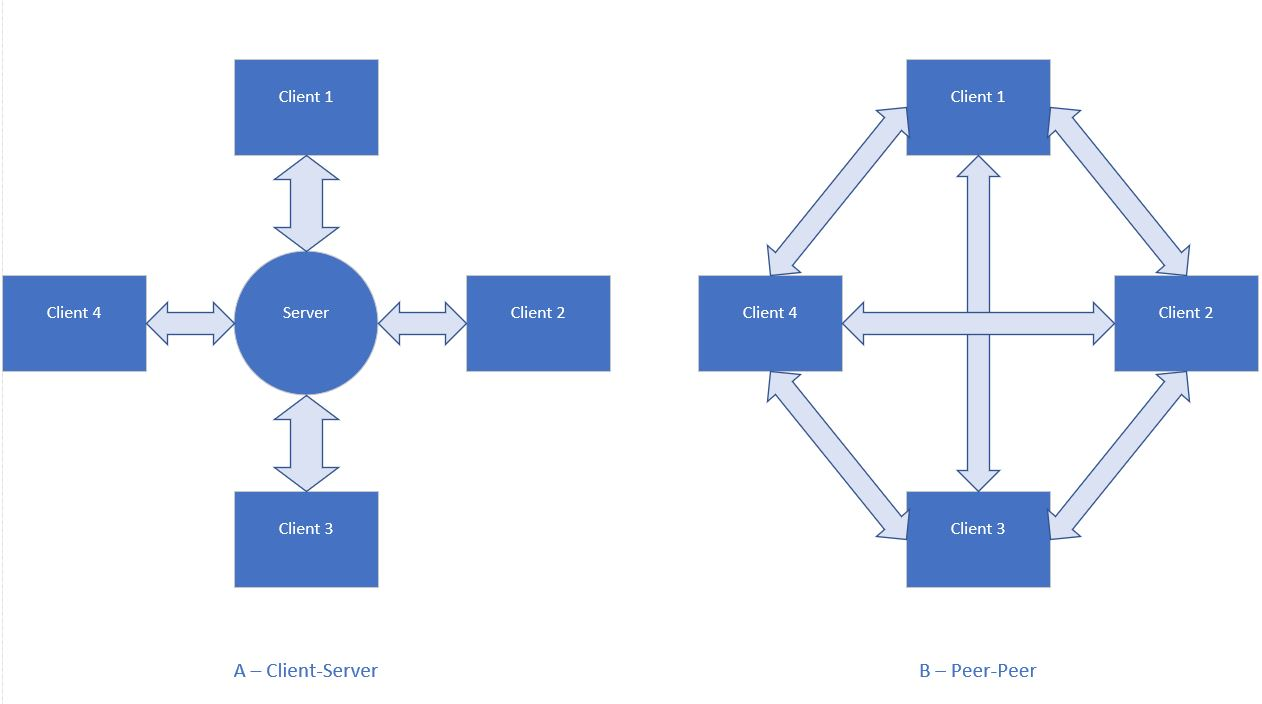
\includegraphics [width = 9cm, height = 5cm] {NetworkArchitecture.jpg}}
\caption{Example of a Client-Server and Peer-Peer Architecture}
\end{figure}

Another type of network architecture exists which has one server serve multiple clients, client-server(Fig. 1). In this type of architecture, one node is designated as the server,
and all authoritative communication is handled through it before being sent to the clients[6]. As noted in Fig 1, we can see that any number of clients may connect to the server
at any one time, and clients do not have to be fully connected since the server is the authoritative source. The client-server architecture will be the target of our testing methodologies
and framework. Although peer-peer has its own valid use cases, it is not appropriate for a centralized simulation and would likewise necessitate a different approach to testing, and thus,
the remainder of this paper will serve a client-server architecture.

With the type of architecture selected, the only remaining task is to introduce the mechanism by which one node communicates with another node. For example, we must answer
the question of how Client 1 and send and receive information from Client 4. Clearly, given that we need to have a centralized simulation, that information must pass through 
the server. The only remaining question is how the server is not only connected to each client, but when that information is to be relayed. There are generally two methods of transmitting
data to and from clients: unicast or broadcast[6]. Fig. 2 demonstrates a high-level overview of the two transmission types. 

The main distinction being that unicast allows one node to initate and send some data to a different node while broadcast allows a node to send information to all other nodes at the same time. 
Intuitively, this implies that an unicast approach would have to initiate and conduct as many transactions as there are nodes. Naturally, this does not happen simultaneously and given sufficient nodes,
the probability that the simulation comes out of sync between clients increases. Therefore, since there is only one true simulation in the system, it becomes advantageous to leverage the ability of 
to broadcast a message simultaneously to all other nodes. The advantage of on-time dispatching of data becomes ever more noticeable when dealing with the type of software we will discuss in the case study, multiplayer
games. 

\begin{figure}[htbp]
\centerline{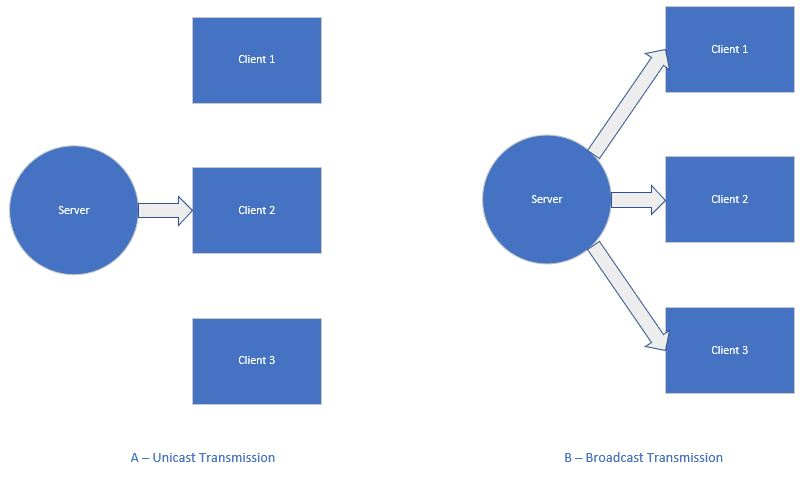
\includegraphics [width = 9cm, height = 5cm] {TransmissionArchitecture.jpg}}
\caption{Example of Unicast and Broadcast Transmission Architecture}
\end{figure}

\subsection{3D Rendering at a High Level}

In the real world, we have object which we can look at and interact with. When such objects are created in a 3D renderer,
some data must be modeled about the object. For simplicity, we will only consider a Cartesian coordinate system(Fig 2), in which points are mapped 
by numerical coordinates along three perpendicular lines(axes). Intuitively, the positional information may be expressed in terms of a displacement 
along each one of the three axes (X, Y, Z). As such, a simple vector with three components can encode this information(Fig 1.): 

\begin{figure}[htbp]
\[ (V_{x}, V_{y}, V_{z}) \]
\caption{Vector Used to Encode Position}
\end{figure}

\begin{figure}[htbp]
\centerline{
\includegraphics [width = 9cm, height = 5cm] {fig1.png}}
\caption{Example of WebGL Coordinate System}
\end{figure}

However, simply listing the position is not sufficient in order to accurately map the object in space. An object may be rotated 
around its position. Fig 2. shows a simple example of a car being rotates about the Z axis. The simplest method by which this information can be encoded 
is to use another three component vector to keep track of the roation around each axis, and then apply each rotation to each axis in a cascading fashion. 
This is commonly known as an Euler Angle, which is intuitive to use, but not sufficent enough in our use case due to the possibility of gimbal lock. 
In short terms, gimbal lock can occur when two axes are in a parallel configuration to each other, which would force an otherwise single axis rotation to instead 
become a composite rotation. 


\begin{figure}[htbp]
\centerline{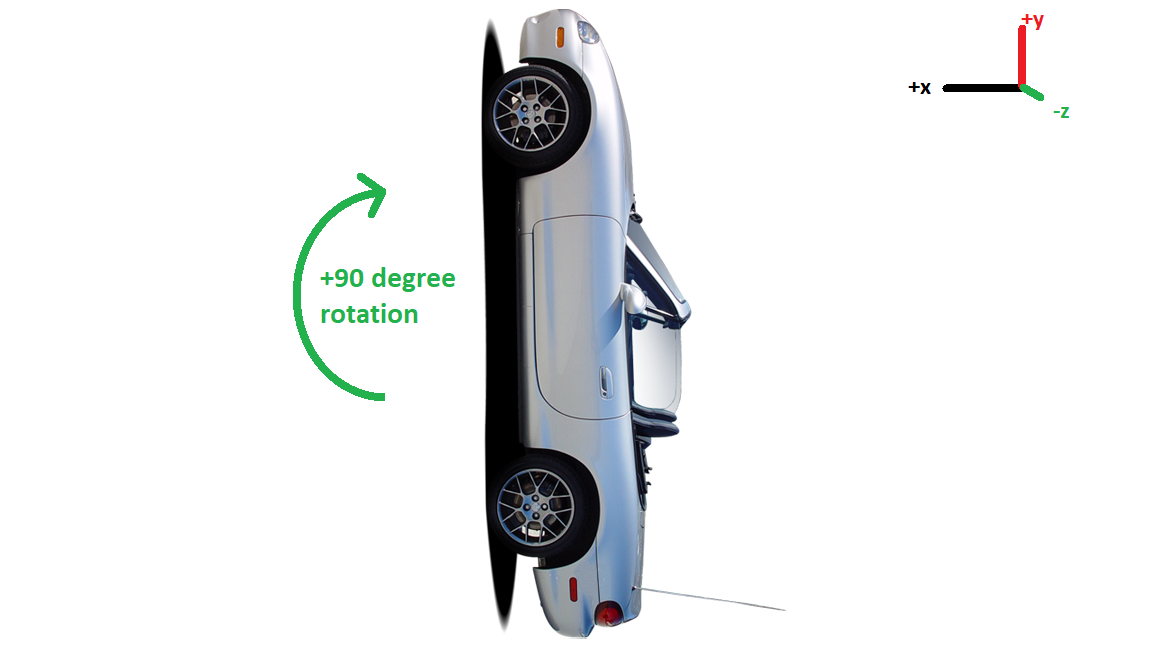
\includegraphics [width = 9cm, height = 5cm] {fig2.png}}
\caption{Example of Rotation Around the Z Axis}
\end{figure}

The conventional solution to this problem is to discard the Euler Angle representation of rotation in favor of using quaternions. 
For the purpose of this paper, we must only know that an equivalent description of orientation can be encoded in a quaternion,
but without the gimbal lock limitation which would cause rotation behavior should it occur. In short, this quaternion may be expressed as a four dimensional
vector, similar to the one expressed in Fig 1., but with an extra component, \textit{w}. 

At this point, we have all of the necessary information to encode a static object in our game world, yet there is one more attribute which
must be implemented: velocity. Consider that an object in our game is in motion, assume it is moving along the X axis. If we have enough snapshots of its location,
then we may be able to render its path up until the current snapshot. However, consider what happens until the next snapshot is received; we will have no idea about the object's path. 
In order to circumvent this, information about how fast the object is moving may be encoded such that an extrapolation between snapshots may occur. This velocity attribute 
is split into two segments; the liear velocity, which is the change in position across the Cartesian system, and angular velocity, which is the change in orientation. 
Each one of these attributes may be encoded in a three dimensional vector(Fig 1).

\begin{figure}[htbp]
\begin{equation}
\text {Position:} (V_{x}, V_{y}, V_{z})
\end{equation}
\begin{equation}
\text {Orientation:} (V_{x}, V_{y}, V_{z}, V_{w})
\end{equation}
\begin{equation}
\text {Linear Velocity:} (V_{x}, V_{y}, V_{z})
\end{equation}
\begin{equation}
\text {Angular Velocity:} (V_{x}, V_{y}, V_{z})
\end{equation}
\caption{Complete Object State}
\end{figure}

Fig 6 shows our final object state. This will be our basic building block when we will discuss the protocol in detail, 
as this will become the data packet which updates clients on the state of the simulation and the objects therein. 

\subsection{Game Model}

The protocol workflow has been described at a very high level, but it is agnostic to the specific game and the rules associated with it. The 
player is modeled by a tank object. This tank object has a few properties associated with it: alive, outOfBounds, score. The alive state 
dictates whether the tank is on the playing field - given that in our rules we have established that being shot simply leads to a respawn, 
this state is only used to indicate that a respawn must occur and that the other player's score is incremented. The outOfBounds attribute is true 
when the player steps outside of the game field, which leads to alive being set to false and score being decremented. The score attribute 
keeps track of the player's current score. 

A keen observer would note that a player's tank has many more attributes that those listed above. Rezin et al [3] utilized model checking 
on a multiplayer game, and they came up with an attribute list which contained all variables that would change over the course of the game.
The attributes are tied into parameters, which are constants set at the beginning of the game. For example, a player's tank can be modeled
as a parameter with attrbutes X position, Y position, Z position, lookAt, score, alive, outOfBounds. The limitation of using this approach is that 
if an object's position is utilized in checking the model, the list of all possible state combinations would be too large to ever compute due 
to the size of the game field having granularity in the tens of millions and the total number of possible lookAt locations also being in the millions.

With these considerations in mind, model checking has also been overlooked in favor of utilizing automated testing to test the 
game directly for consistency in its rules. One thing of note is that the formal definition of the game rules for example, a valid x coordinate,
is syntactically equivalent to the check the game logic would perform; therefore writting a model checking program is redundant in this specific 
case. Fig 11 shows the formal definition along with the implementation of the rule.  

\begin{figure}[htbp]
\[ (W_{xmin} \leq T_{x} \leq W_{xmax}) \]
\[ !(playerTanks[k].obj.position.x < xMin ||\]
\[ playerTanks[k].obj.position.x > xMax) \]
\caption{Formal Rule and Implementation of Valid X coordinate}
\end{figure}

\section{Approach}
Our approach is to develop a generalized framework for NodeJS will combine abstract testing of models, unit testing, and functional testing into a single, yet modular, 
utility. The effort of functional testing will involve the synchronization of timing of outputs from the server as well as the clients involved. The testing utility 
should be distributable just as the software being tested and a means of distributing and launching a test should be runnable from a single test location. Any data and 
any results of a test run should also be collected and delivered to the single test location where it will be analyzed and classified as either a success or failure. 
Current design will feature the integration of the Labstreaminglayer tool and a Labstreaminglayer server. This tool will allow for the collection of any data or output 
deemed necessary for a given test. It will allow for record sub-millisecond timing of events from multiple machines over a local area network.

For the goal of developing and testing the game locally on one machine, we will also be able to leverage the fact that it is built to run in the browser on
an interpreted language to run test suites end to end. Firstly, we will investigate an approach similar to Ariyurek et al[2] in order to develop an automated 
system to test the application as well as to automatically find problems with it. Secondly, the fact that the application in its unobstructed build state will have
its internal state visible and inspectable from the outside. That is to say, if we were to run multiple client simulations concurrently, we would be able to inspect 
the state of the simulation on each one of the said client machines independently. This would allow us to inspect the correctness of the model in real time from the 
perspective of each client. Likewise, the fact that we could control each client independently, we will be able to gauge the susceptibility of the simulation to erroneous 
or malicious data by willfully introducing it to one client, and checking if the erroneous data was propagated to the other clients.


\section{Implementation}


\subsection{Automated Client-side Testing}

The first testing scenario we will consider is to allow the system to automatically play the game in order to test a set of pre-defined set of actions.
For example, let's assume that we may programatically interact with the simulation directly in at least one of the client instances. With the system having control over a client simulation, 
we can individually test the different interactions with the simulation. This type of autmated testing could be invoked on an individual developer's 
machine in order to test each function of the system as its being developed or modified. If the simulation has a visual representation, then perhaps it will be beneficial to 
visually show any changes to the simulation state to the viewer as the tests are being invoked.  

Consider the architecture diagram in Fig. 1, wherein each client has a two-way connection to the server. The client may push an update to the simulation state, and likewise each
client can receive the updated state at any time. If we are to perform an automated functional test, then it would be sufficient to tap into one of the clients, and simply invoke 
some change in that client. However, while this may be sufficient to verify that operability of the functions pertaining to a client, it does not guarantee that the entire system 
is indeed working as intended, namely that all other clients are receiving and rendering the updates correctly. Fig 8. shows our proposed approach to this problem. Note that a "Testing Framework"
entity is created, which is communicating to each client, and would have the ability to programatically invoke a client change, and likewise to programatically listen to any changes in each client.
With these capabilities in mind, the framework would be capable of provoking a change in a client and then verify the change in all other clients for correctness. 


\begin{figure}[htbp]
\centerline{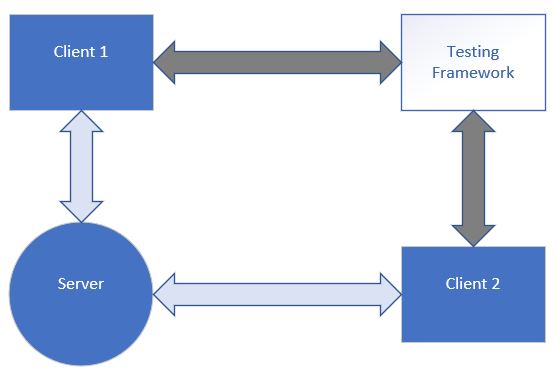
\includegraphics [width = 6cm, height = 6cm] {images/ClientSideFrameworkDiagram.jpg}}
\caption{Architecture with Client-side Testing Framework}
\end{figure}


\subsection{Automated Full-stack Testing}

To be developed 


\subsection{Remote Testing}

\subsubsection{Core RPC Services}Remote testing of the target application is achieved through an adaptable and extensible pair of RPC services. Two APIs, 'Data' and 'RemoteCtrl', that enable remote testing and they are capable of being updated and expanded quite easily as the application's range of behaviors grow during its lifetime. Each API service is defined in an IDL(Interface Description Language) file. Each defines the a service's name followed by generic a list call signatures of the functions that shoould be exposed by the service. The IDL offers several plain data types such booleans, floating points, a string type, and signed integers of the typical varying bit-widths. Basic C-style structures and enumerations may also be defined to add versatility to the services defined types.
\subsubsection{RPC Adaptability}As the application grows and new types of interactions and information need to be handled, the same pair of IDL need only minor editing by the maintainer. Automatic generations scripts may be rerun at each stage of changing demand. The resulting output is a fully-formed supporting library in the target programming language of choice for, both, the client and server sides of each RPC service. The RPC-server half of each API is included and/or linked to from the simulation's server to allow both services awareness of and access to all necessary data of the simulation's clients. In the event of new or changing data types, the client simulation needs only to be rebuilt in the case of a compiled-language and no changes are required for interpreted languages. In the case of new or changing functions, the auto-generated RPC handlers need only be given function bodies by the tester. Building remote testing utilities for the simulation is easily done thanks to this process, as there are no dependencies between the programming language of the simulation's server and the RPC client. The RPC service itself manages all translation between native data types of the server and it's RPC client. This means the RPC service manages the serialization/deserialization and transport of all function arguments and return values, byte-order translation between differing host hardware, and member alignment between differing host operating environments. All these features allow for a simulation written in javascript, C++, Java, Python, C\#, etc. to agnostically cooperate with any client written in any other supported language and host operating environemnt.
\subsubsection{Distributibility}With an underlying TCP or UDP transport layer, this remote testing strategy allows for a wide range of geographical testing configurations to be thuroughly explored. Testing and examination of the system may be performed in a close-proximity LAN configuration, or the simulation server and its clients may be much more georgraphically separated, communicating over the Internet with one another and the testing client itself.


\section{Case Study}

With the all of the prerequisite work complete, the implementation of the testing framework for the game and protocol will be discussed. For reference,
the project code is located at (https://github.com/spac3nerd/CSI-5390Proj). The NodeJS server 
will need to run both traditional HTTP transactons and socket transactions. The HTTP transactions are used to ask the server if 
there are any open spots in the game, and whether access is granted to a new player. If access is granted, then the server will return 
an unique token to the client with which a socket connection can be requested. The client then requests entry into the game 
with the token and a tunnel is established between the client and the server. Fig 8. shows the game being played by three players, with
the blue tank being controlled by the current instance.  


\begin{figure}[htbp]
\centerline{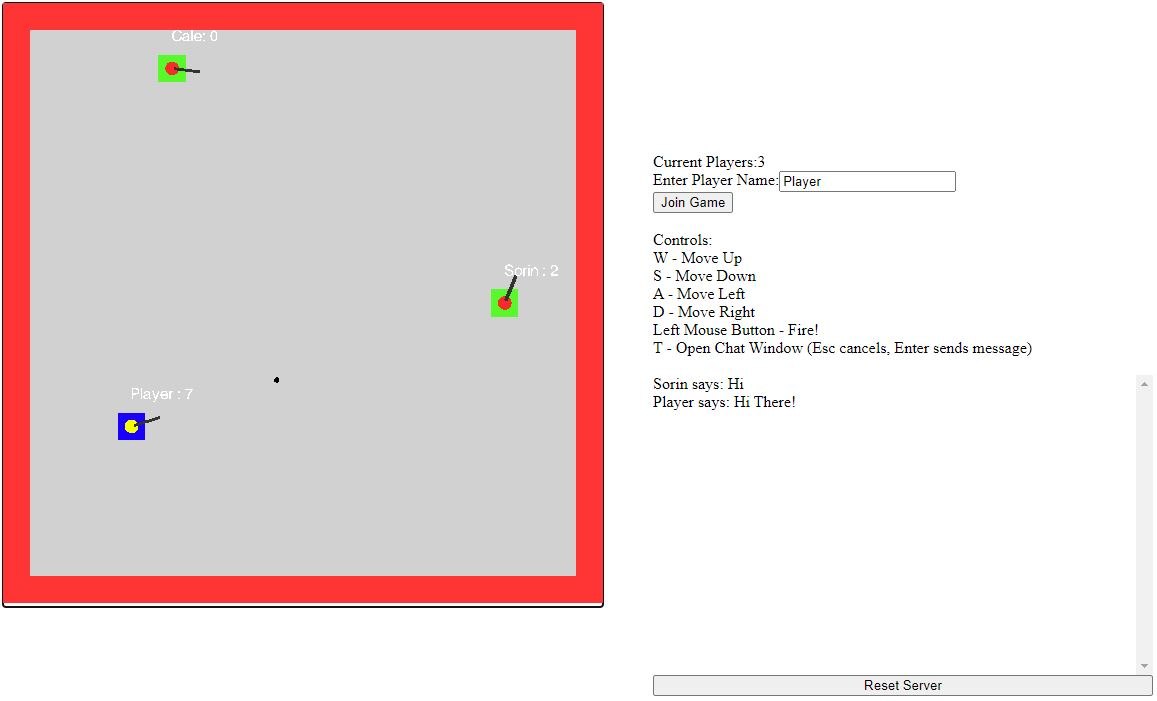
\includegraphics [width = 9cm, height = 5cm] {GameScreenshot.jpg}}
\caption{Screenshot of the Game with Three Players}
\end{figure}

Note that each player has his own score count,a representation of all of the other tanks as well as any bullets which were fire, and finally, a chat area
in which any player may type a message to send to all other players at any time. To The full list of rules to the game are as follows:

\begin{itemize}
  \item A Player may move his own tank in any direction at any time.
  \item A Player may aim the tank and fire a bullet at any time.
  \item If a Player's bullet intersects another tank, that tank is destroyed and a point added to Player.
  \item If a Player's tank reaches the red area, their tank will be destroyed and a point deducted.
  \item A Player may send a message to all other players at any time.
\end{itemize}

With all of NodeTank's rules layed out, we have the knowledge necessary to start building up the types of test cases and tests we require. 
In the following sections we will cover the specific testing implementations with the goal of addressing the problem of rigorously testing NodeTank, however, these techniques 
are easily applicable to other multiplayer games built on the NodeJS platform. 

\subsection{Automated Client-side Testing}

As mentioned in the Implementation section, each client has either the ability to affect the simulation in some fashion, or is at least capable of receiving an updated
version of the simulation. In the case of NodeTank, each client is responsible for controlling one tank according to the aforementioned rules of the game. As previously mentioned,
instead of simply unit testing in the traditional sense(isolating one function at a time), but instead attempt to perform a test based upon some use case or rule of the game we will
 benefit from being able to not only test the individual action on one client, but across all clients. Let's take the first rule of the game for example and infer the implications for the entire system 
 of that action being actionable. If a Player A is to move in any direction, then clearly that movement must be rendered in Player A's simuluation at the very least. To allow for interactivity, 
 the movement must be rendered in the simulation of all other players, which implies that the server must correctly receive, process and send a correct update to all players. 
 
 The proposed implementation called for a testing library to be written, which caters to the peculiarities of a case such as NodeTank while providing generalized functionality for all 
 applications of the same architecture. Recall the class diagram in Fig 8. layed out the server-side and client-side classes utilized by the game. The authors have implemented a framework
 under a class entity called "NodeTankTesting", which is coupled into one more more instances of the client-side. The applied changes are visualized in the Fig. 9 daigram. At a high-level,
 the framework provides mechanisms to start up an instance of NodeTank client in the browser, register tests, programatically control a player and assertions to verify the state of each client. 

\begin{figure}[htbp]
\centerline{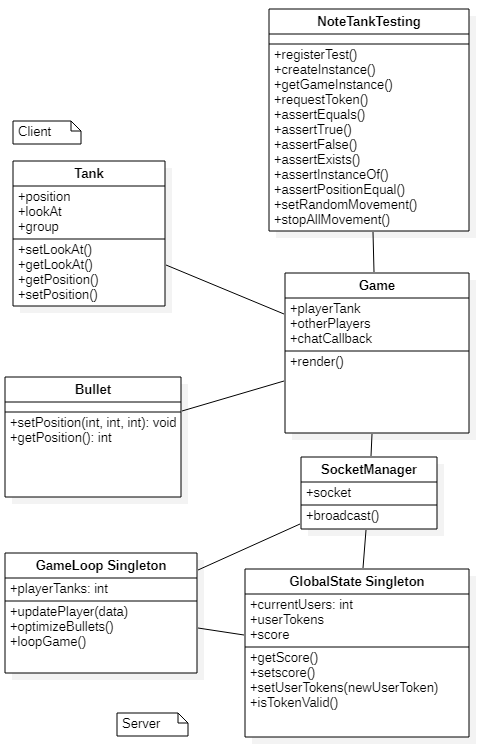
\includegraphics [width = 6cm, height = 9cm] {classv2.PNG}}
\caption{Modified Class Diagram with Testing Framework}
\end{figure}

This testing framework relies on the ability to access the internal state of any client instance of NodeTank. The reader may be interested to know that the author of NodeTank 
elected to utilize the prototype pattern, which is a JavaScript design pattern which allows for great control over inheritance while exposing any closures to outside observers[7]. For example, 
let's take the Game class from the client-side in consideration. In Listing 1, we can see that the variable "game" is defined into two sections: there is a function declaration, whose body functionally 
behaves like a constructor, and a prototype assignment, which is a set of methods inherited by all instances of game. The keen reader will note that this is not quite the same classical inheritance
mechanism utilized by languages such as Java, however we will continue to refer to them as classes as functionally they behave similarly enough.

\begin{lstlisting}[language=JavaScript,caption={Snippet of the Game Class}]
    game = function(canvas, socket, token, name) {
		this.canvas = canvas;
		this.socket = socket;
		this.token = token;
		this.name = name;
		this.initCallback = undefined;
		//...
	};

game.prototype = {
    //set up an instance of the game
    init: function(callback) {
        this.initCallback = callback;
        this.configSocket();
        console.log(this.name);
        this.socket.emit('joinGame', {
            token: this.token,
            name: this.name
        });
    },
\end{lstlisting}


The benefit of the prototype pattern is that we are able to inspect the internal state of any game instance running in the brwoser, and we are also able to programatically induce 
any inputs such as movement, firing and entering new chat items. Fig 11. is an example of inspecting the entire instance of NodeTank and the position of the player tank programatically.

\begin{figure}[htbp]
\centerline{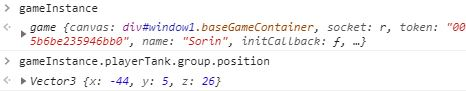
\includegraphics [width = 9cm, height = 2.8cm] {GameInspection.jpg}}
\caption{Inspecting an Instance of NodeTank}
\end{figure}

Now that we have a handle to a game instance, we can begin to write some test cases which will allow us to test every client-side functionality of the game. For example, before a player can
connect to the server, the connection must first be negotiated over a HTTP call. The testing framework has a builtin to send the negotiation request along with the player's desired name, and if the 
server is not at the maximum player capacity, it will respond with an unique token which will be used from thereon as an identifier. In order to test this functionality, we can programatically request
the new connection and verify that a token was issued (or denied) as expected. In Fig 12. we can see the implementation of this test - note that "t" refers to the testing framework and that the "requestToken"
function requires that a callback be provided, which is called whenever the response for the token request is received. 

\begin{lstlisting}[language=JavaScript,caption={Snippet of Test Case for Requesting a Token}]
    let id2 = t.registerTest("testCase2");
    let test2 = (resolve, reject) => {
        t.requestToken(player1Name, (token) => {
            if (t.assertExists(token)) {
                t.passTest(id2);
                resolve ? resolve() : null;
            }
            else {
                t.failTest(id2);
                resolve ? resolve() : null;
            }
        });
    };
\end{lstlisting}


However, a problem remains with this approach in that the test case will work as intended if manually invoked in isolation. Consider that the call itself is asynchronous - we cannot block the 
main (and only) thread on the client-side while we wait for a response to come back from the server, doing so would pause the client-side simulation at every network interaction and there would be no interactivity! 
Suppose that we wish to have an entire suite of tests, and that some of those tests rely on the previous test completing before being invoked. If a string of synchronous function calls would be utilized
in testing, then we would have no mechanism by which to ensure that test B is only called after test A completed if test A is at all asynchronous. Therefore, a more intelligent design pattern must 
be leveraged in order to allow the framework to test all cases automatically. Fig 13. showcases the desired sequence diagram for launching two tests at the correct time without blocking the main thread. 


\subsection{Remote RPC Services}
Our implementation of the \textit{Data} and \textit{RemoteCtrl} APIs were built upon a tool known as Thrift, originally created by Facebook, but now managed by Apache. The RPC services contain several functions, between the two of them, for retrieving and executing testing and control operations including \textit{GetTokenByName}, \textit{GetPose}, \textit{SetMove}, \textit{Fire}, \textit{StartDataServer}, \textit{ExecuteTest}, \textit{GetTestResults}, and \textit{GetTestCases} to name a few. The RPC handlers of each RPC services are setup within \textit{gameCore}, the game's primary server. From here, they are pointed to the appropriate handling functions. These handlers allow for the computational logic of the services to access all the necessary information from \textit{gameLoop.js}, \textit{global-state.js}, and \textit{socket-manager.js}.

\subsubsection{Remote Testing Service}
Within \textit{gameCore} the RPC host objects are setup each to operate within their own thread, alongside the game's primary servers.

\begin{lstlisting}[language=JavaScript,caption={In this example, the thrift is used to create a server for the  'dataInterface' service. It then lists two skeleton functions to handle 'GetGameData' and 'ExecuteTests' functions.}]
dataServer = thrift.createServer(dataInterface,{
  GetGameData:     function(){
      let game_data = { /*meaningful code*/ };
      return game_data;
    },
  ExecuteTests:    function(arg1,arg2){
      // Custom handler code goes here
    },
    .
    .
});
dataServer.listen(9091);
\end{lstlisting}
This RPC server instantiation serves as the primary hook into the innards of the game, and is how the queries into the internal game objects' states are achieved.

\subsubsection{Remote Control Service}
The control service is implemented in the same manner. Instead of focusing on extracting information from the server, the remote control service operates on the server's internals by calling its internal functions, even supplying arguments to them from the outside. Functions exported from the module in \textit{socket-manager.js} are at the disposal as well, including those for making websocket calls to client instances. This extends the reach of the control service even further, allowing it to pass commands along to client code, for example, initiating the client to perform functional tests upon itself and to alert the server after it has finished. The final type of control interaction provided by the service is launch the remote testing service's server, which is not running by default. This makes the the control service client a dependency of any remote testing client.

\subsection{Remote Control Service's Supporting Role}
The additional goal of the testing framework alongside the remote testing utilities to to support extended periods of software testing. The motivation for this being to allow testers to discover unintended and most likely unwanted effects of long-term execution times of their software. Through manual testing of NodeTank, we discovered that spent bullet objects were not being destroyed after leaving the rendered region of the game. This build up, over time, led to considerable sluggishness. It is these emergent properties and behaviors that are often hard to test for with a human in the loop, and can go undiscovered for quite some time. To solve this problem we had proposed the idea of implementing an Agent play the NodeTank game for extended periods of time that would otherwise be unrealistic to expect of a human player. Allowing the game to run for extended periods of time with external interaction would allow for fuller and more expansive sweep of the ranging states of gameplay. Traditionally in reinforcement learning, an abstract set of game states would be established, and for those states, corresponding actions that would be appropriate for a player to take reinforced by a reward. This mapping of states and actions would be stored in what's known as a Q-table. As the agent explores various actions in the environment, it updates the values in the Q-table to reflect those actions that yielded the maximum cummulative reward. In the case of gaming, especially those rendered in 3-dimensions, there is substantial state explosion that occurs when taking into account all of the possible positions, orientations, objects, and object interactions. Storing these states and actions becomes very impractical very quickly. To overcome this problem, the Q-table will be replaced with a deep-query neural network, or DQN. The additional training time required for a DQN is a trade-off made for the constant memory that would otherwise grow exponentially with a Q-table. Additionally, the DQN would, after being trained, be able to select actions in response to environmental observations it has never seen before, which is another major advantage over the traditional Q-table. Pushing environmental information to and receiving player input from the DQN is a major intended role of the remote control service.
\paragraph{Injecting user input}
The remote control service has several functions that allow for injecting input that would otherwise come from a player, directly into the \textit{gameLoop.js} singleton. This includes RPC calls for positional movement, rotating, and firing the NodeTank tanks. It is the inputs to these functions that would be the direct outputs of the DQN's fully-connected layer. This output would be fed to the remote control service's functions following each of the DQN's action predictions.
\paragraph{Extracting the rendered environment}
To further facilitate the training of this agent, the remote control service is meant to forward environmental observations to the agent. These observations are in the form of a snapshot of the most recently rendered frame of the game. This image is encoded in a base-64 string and sent to the server where it waits to be requested by the remote control service. After receiving and decoding the base-64 string, the image would be scaled down to more ideal dimensions for input into the DQN. As this observation data propgates forward through the convolutional layers, more and more features are extracted before finally being flattened and fed into the full-connected layers of the network to decide upong the most ideal actions to output. The results of those actions amount to a reward in the game's environment, in our case, the players score which will drop if the player is hit by an enemy, and rise if the players hits an enemy. In actual implementation, the environmental observations, chosen actions, and environmental reward are stored in what's known as a \textit{replay memory}. This \textit{replay memory} is vital to the stable learning of the DQN, as memories have to chosen in random batches for processing by the DQN to alleviate the high temporal correlation of processing back-to-back frames of gameplay.

\begin{figure}[htbp]
\centerline{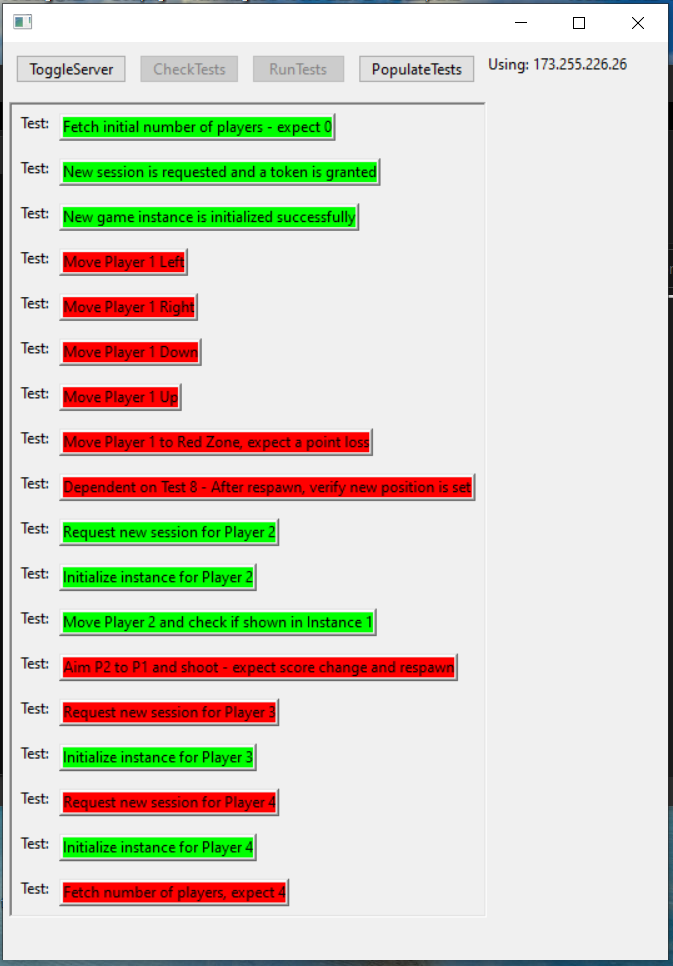
\includegraphics [width = 5cm, height = 6cm] {images/remoteTesting.PNG}}
\caption{Example of a testing application built using our remote testing APIs. This instance can cycle between multiple remote simulation servers. It populates a list of available unit tests available on that server, can execute them, and then presents the results to the tester by highlighting list items in green or red to indicate pass or fail respectively.}
\end{figure}



\section{Conclusion}

To be developed 

\subsection{Future Work}

\section{References}
[1] A. Valadares, “Aspect-oriented architectural style for distributed interactive simulations”, 2016, 
Available from ProQuest Dissertations \& Theses Global. (1881527059). 
Retrieved from https://search-proquest-com.huaryu.kl.oakland.edu/docview/1881527059?accountid=12924

[2] S. Ariyurek, “Automated Video Game Testing Using
Synthetic and Human-Like Agents”, 2019, Available: https://arxiv.org/pdf/1906.00317.pdf
	
[3] R. Rezin, ”Model Checking in multiplayer games development”, Innopolis University, 
2017, Available: https://arxiv.org/pdf/1712.01207.pdf

[4] R. Hofer “DIS Today”, 1995, Available:
https://ieeexplore.ieee.org/stamp/stamp.jsp?arnumber=400453

[5] J.Peusaari, “Distributed Issues in Real-Time Interactive Simulations”, Department of Technology Lappeenranta University of Technology, Finland,
 Available: https://ieeexplore.ieee.org/abstract/document/5361761
 
[6] J. Smed, “Aspects of Networking in Multiplayer Computer Games“, Proceedings of International Conference on Application and Development of Computer Games in the 21st Century, Hong Kong, 2001,
Available: https://www.researchgate.net/publication/269251176\_Aspects\_of\_Networking\_in\_Multiplayer\_Computer\_Games

[7] A. Osmani "JavaScript Patterns", Book, 2012, Available: https://addyosmani.com/resources/essentialjsdesignpatterns/book/
\end{document}

